In this section we conducted our experiments on a heterogeneous infrastructure like Amazon EC2~\cite{amazonEC2} and on a homogeneous infrastructure like DAS-4 (the Distributed ASCI Supercomputer 4)~\cite{das4}. DAS-4 is the Dutch Computational Infrastructure, a six-cluster wide-area distributed system designed with research purposes.  We compare the degree of SLA fulfillment and resource consumption for each one of the provisioning algorithms included in ConPaaS.

Note that, since DAS-4 is a homogeneous infrastructure, the profiling techniques were only evaluated on a heterogeneous platform like Amazon EC2. 


\fixme{Include all the assumptions ??} 
\corina{I guess only the important ones (but what kind
of assumptions were you thinking about?}
\fixme{I did not mention the size of our checking window: 5min, 5min also  }
\corina{I think we should mention that.}

\subsection{Testbed configuration}

As a realistic and representative scenario, we deployed Mediawiki application using ConPaaS on both clouds, and we ran the Wikibench tools utilizing Wikipedia workload traces.  

To provide the Wikipedia services, an initial configuration was composed of 4 VMs, and 1 VM to host the Wikibench tools. The 4 VMs include a PhP service manager, a FPM-PhP agent, a web server and a http-proxy agent (in the same VM), and a MySQL service to store the English Wikipedia data, as explained in Section~\ref{wikipedia}.

Thus, the provisioning system will scale out and back the number of VMs hosting FPM-PhP agents to guarantee the SLO (Service Level Objective). Initially, we fixed two SLOs one of 700ms (milliseconds) at the service's side and another of 1500ms at the client's side. Our measurements shows the behavior of the Wikipedia services during 24h under a workload generated from real access traces. Note that, our experiments only focus on the average of PhP response time and the resource consumption of our algorithms. The response time of static file requests is not evaluated due to the lightweight nature of the static files employed by Wikipedia articles. 

\subsection{Homogeneous Infrastructure}

Our experiments on DAS4 relies on OpenNebula as Infrastructure-as-a-service (IaaS). To deploy the Wikipedia services, we used small instances for the PhP service (manager and agents) and a medium instance for the MySQL service (agent). OpenNebula's small instances provision VMs equipped with 1 CPU of 2Ghz, and 1GiB of memory, while medium instances are equipped with 4 CPU's of 2Ghz, and 4GB of memory.

Figure~\ref{naiveDas4} and Figure~\ref{historyDas4} depict the degree of SLA fulfillment for the naive and history-aware algorithms, indicating the average of response times obtained during the execution of the Wikipedia workload trace. The results show how the naive provisioning algorithm tends to generate more SLA violations due to its excessive reactive behavior. These violations are comprised between \emph{700ms} (see the yellow Line) and \emph{1500ms}(see the red Line) response time values. As we mentioned, this algorithm is an easy target to flash crowds effects, as new VMs can be added or removed  to handle sharp and sudden variations in the workload. In contrast on Figure~\ref{historyDas4}, the system performance (\emph{i.e.,} response time) do not fluctuate greatly showing a more stable behavior during the whole experiment. As well we also appreciate a reduction in the number of SLA violations regarding the total amount of PhP-served pages.

% (a 1\% less) 

\begin{figure}

\begin{center}
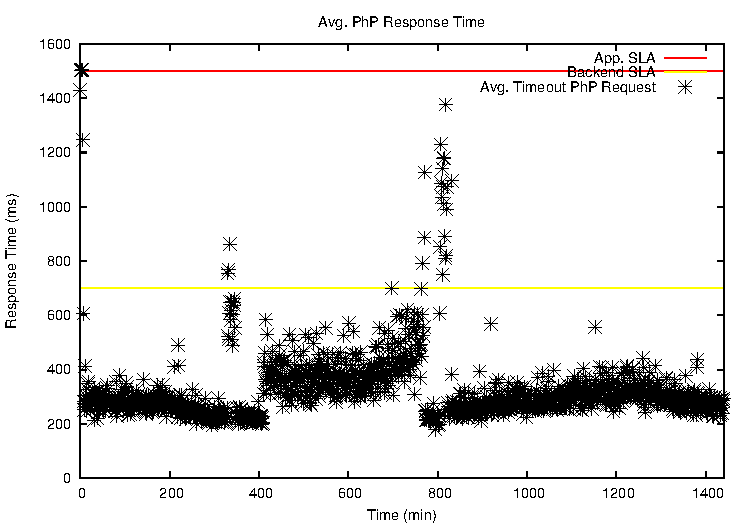
\includegraphics[width=0.49\textwidth, height=6cm]{./images/homogeneous/avgTimeout_PhP_naive}
\end{center}
\caption{PhP resp. time on DAS4 -- Naive.}
\label{naiveDas4}
\end{figure}

Nevertheless to better understand the behavior of both algorithms, we may focus on the resource consumption, as depicted on Figure~\ref{resComDas4}. Firstly, the excessive reactive behavior of the naive algorithm is again illustrated at the interval \emph{t=350min} and \emph{t=820min}, where two scaling operations under-provision the system during a short period of time. These provisioning decisions provoked fluctuations in the system performance that incremented the financial cost, and therefore throughput alterations. When using the history-aware algorithm, the system makes provisioning decisions by analyzing workload's trend during a considerable interval of time. Scaling actions are only triggered when having constant alterations in the Wikipedia workload, providing a more efficient resource usage. Indeed, the workload alterations depicted on Figure~\ref{workload}, match with the provisioning decisions made by the history-aware algorithm on Figure~\ref{resComDas4}.

\begin{figure}
\begin{center}
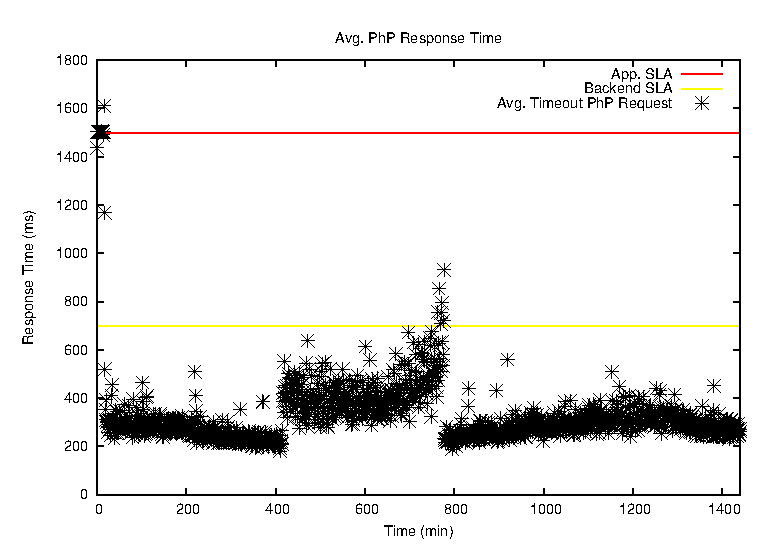
\includegraphics[width=0.49\textwidth, height=6cm]{./images/homogeneous/avgTimeout_PhP_history}
\end{center}
\caption{PhP resp. time on DAS4 -- History-aware.}
\label{historyDas4}
\end{figure}

\fixme{I will run more time the History-aware exp. on DAS4.}

\begin{figure}
\begin{center}
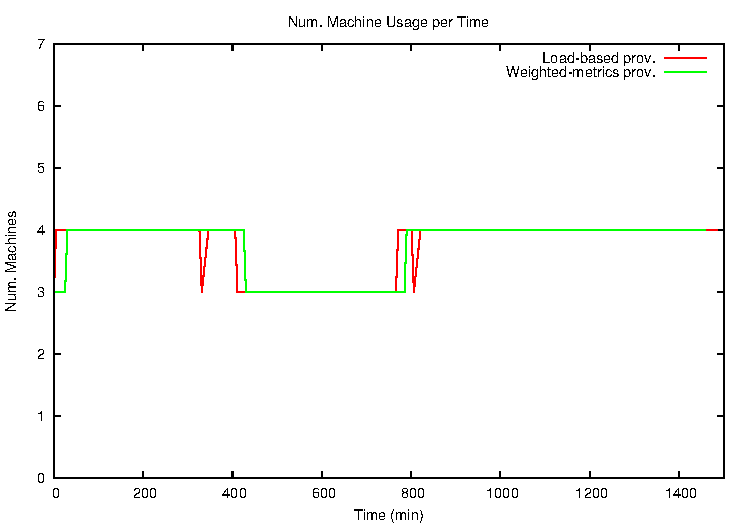
\includegraphics[width=0.49\textwidth, height=5cm]{./images/homogeneous/numMachinesComp}
\end{center}
\caption{Resource consumption on DAS4.}
\label{resComDas4}
\end{figure}

\subsubsection{Discussion}

Using the naive provisioning algorithm, the system performance fluctuates greatly following a pattern similar to the web traffic that increases the number of SLA violations. The reactive behavior of this algorithm triggers scaling actions that affect to the system performance instead of improving it, and as a consequence they are also wasteful in terms of resource consumption. Unlike history-aware algorithm offers an efficient resource usage and a constant performance behavior while meeting the application's SLA. Therefore this algorithm finds the tradeoff between accuracy and cost savings.

Both algorithms are best-effort regarding the SLA fulfillment, and thereby temporal alterations of the workload (with a duration of 5min approx.) cannot be guaranteed. The heterogeneity of the PhP-served pages, containing images and requiring multiple Db queries, and the startup time of VMs are in part responsible of these SLA violations. 

%It avoid to under-provisioning in two occasions  while decreases the number of SLA violation. However, the naive alg. is vulnerable to temporal bursty workload variations (10 min), an increment of SLA violated is caused by under-provisioning operations in conjunction with workload variations. 



\subsection{Heterogeneous Infrastructure}

Our experiments on EC2 used small instances for the PhP service (manager and agents) and  a medium instance for the MySQL service (agent). EC2 small instances provision VMs equipped with 1 EC2 CPU, and 1.7GiB of memory, while medium instances are equipped with 2 EC2 CPU's, and 3.75GiB of memory.

In the following, we analysis the behavior of our algorithms when making provisioning decisions on a heterogeneous infrastructure. Figure~\ref{naiveEC2}, Figure~\ref{historyEC2} and Figure~\ref{historyWeightEC2} show the system performance of the naive, history-aware and profiling-based algorithms, respectively. As depicted on Figure~\ref{naiveEC2}, the performance fluctuates greatly following an irregular pattern when using the naive algorithm. More precisely, two of the three workload peaks caused at \emph{t=300min} and \emph{t=820min}, are explained from the variations on the Wikipedia workload described on Figure~\ref{workload}. However, there is a third peak that corresponds to the interval of time on which the workload trace significantly decreases the number of user's requests. This explains the degradation of the SLA fulfillment as an effect associated to very frequent scaling actions. 

On the other hand, Figure~\ref{historyEC2} and Figure~\ref{historyWeightEC2} show as the history-aware and profiling-based algorithm behave similarly. Even though both algorithms are best-effort, there is an important reduction in the number of SLA violations during the whole experiment. Like on DAS-4, the history-aware algorithm follows a constant performance pattern without having sharp and sudden alterations. Besides, as shown on Figure~\ref{historyWeightEC2}, the profiling-based algorithm has a similar behavior to the history-aware algorithm in terms of system performance, however. The profiling-based algorithm improves the SLA fulfillment in a 11\% in comparison with the history-aware algorithm. Therefore we demonstrate how the use of online profiling techniques although intrusive do not cause time delays or throughput alterations. 

\fixme{performance or responsiveness}

\begin{figure}
\begin{center}
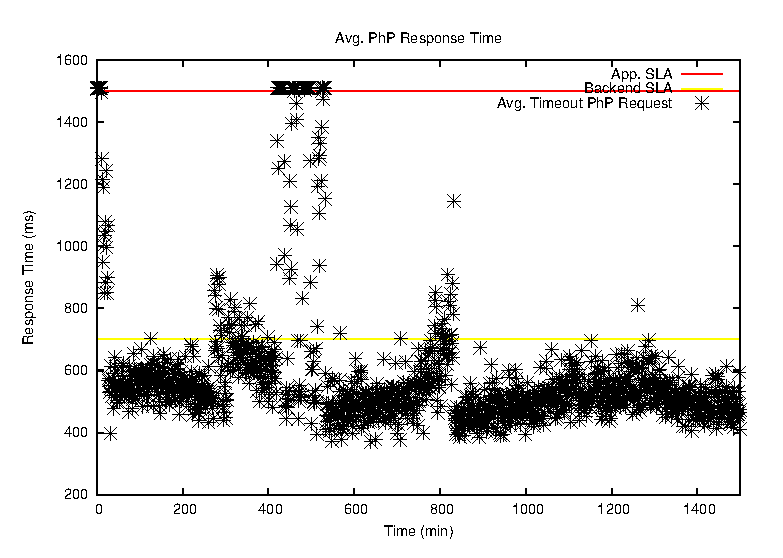
\includegraphics[width=0.49\textwidth, height=6cm]{./images/heterogeneous/avgTimeout_PhP_naive}
\end{center}
\caption{PhP  response time on EC2 -- Naive.}
\label{naiveEC2}
\end{figure}


\begin{figure}
\begin{center}
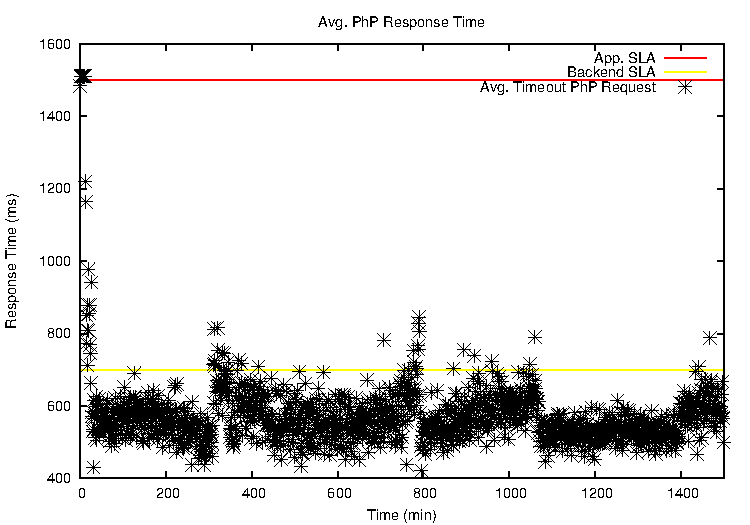
\includegraphics[width=0.49\textwidth, height=6cm]{./images/heterogeneous/avgTimeout_PhP_history}
\end{center}
\caption{PhP resp. time on EC2-- History-aware.}
\label{historyEC2}
\end{figure}

\begin{figure}
\begin{center}
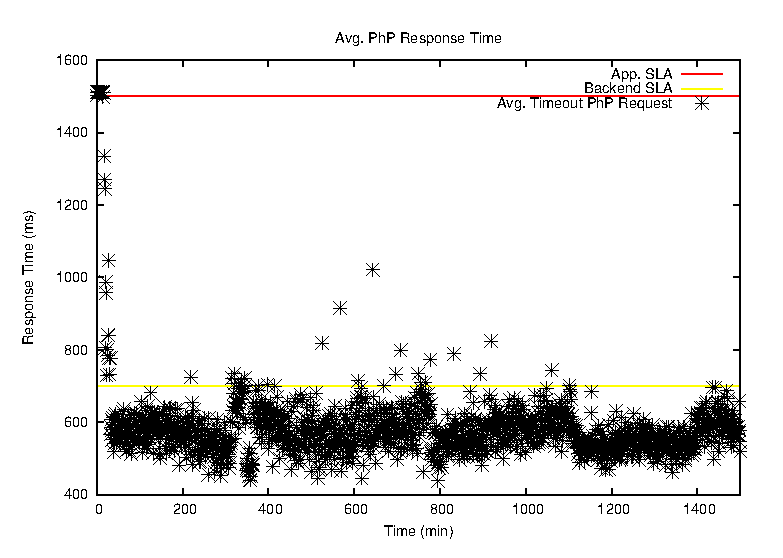
\includegraphics[width=0.49\textwidth, height=6cm]{./images/heterogeneous/avgTimeout_PhP_weightHistory}
\end{center}
\caption{ PhP resp. time on EC2-- Profiling-based.}
\label{historyWeightEC2}
\end{figure}

The resource usage on EC2 presents important alterations as shown on Figure~\ref{resEC2}. When using the naive provisioning, the fluctuations in the system performance are explained as a result of a high frequency of scaling operations. In concrete, these fluctuations caused at the interval of time comprised between \emph{t=400min} and \emph{t=500min} (see on Figure~\ref{naiveEC2}) match with the provisioning decisions made during the same interval of time on Figure~\ref{resEC2}. If we now pay attention to the history-aware, and profiling-based algorithms, their resource consumptions are identical during the whole experiment. Indeed, both algorithms decided to scale out the system during the interval of time comprised between \emph{t=1050min} and \emph{t=1400min}, to prevent future SLA violations. It demonstrates the benefits of using flexible threshold ranges to provide a predictive provisioning mechanism, improving the user experience.


\begin{figure}
\begin{center}
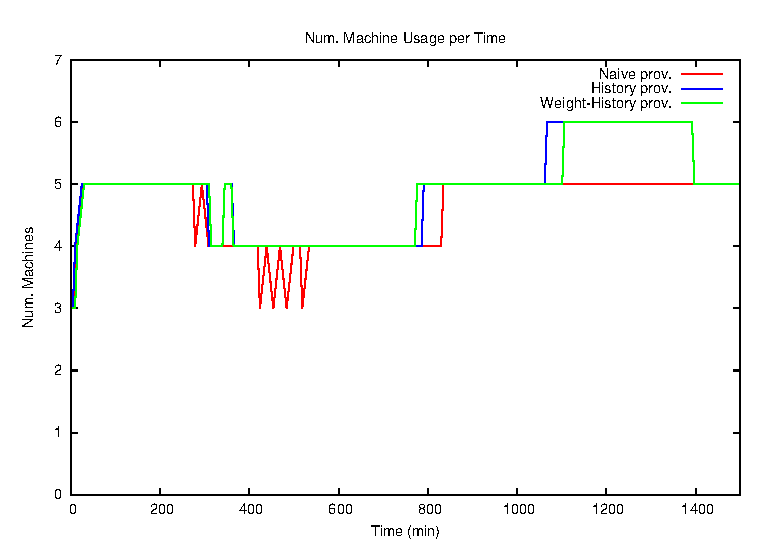
\includegraphics[width=0.49\textwidth, height=5cm]{./images/heterogeneous/numMachinesCompEC2}
\end{center}
\caption{Resource consumption on EC2.}
\label{resEC2}
\end{figure}


\subsubsection{Discussion}

\fixme{Do you prefer this organization for the discussions ? One inside of each type of cloud, and one to summarize. }

\subsection{Discussion}



Generally, the result of our measurements show how the behavioral performance pattern and the resource consumption vary depending on the infrastructures on which we ran our experiments. Different hardware configurations such as those provided by DAS-4 and EC2, offer two distinct scenarios to validate our provisioning algorithms.  In these experiments, we demonstrate how trigger-based provisioning mechanisms can affect the system performance instead of improving it, as well as are wasteful in terms of resource usage. Online profiling techniques, although intrusive, were used without producing performance alterations, in fact they slightly reduced the number of SLA violations in comparison with the history-aware algorithm. We also show the benefits by using history-aware and profiling-based provisioning algorithms which find the tradeoff between the accuracy and cost savings. 

However, in these experiments, the flexible threshold ranges were pre-defined before execution for all VMs. These threshold values have to change depending the type of instance to be provisioned. Therefore, we believe that offline profiling techniques may be used to define these values depending of the type of instance, thus improving the effectiveness of our predictions.

%Today's resource provisioning systems define SLO's based on desirable threshold values for an application (CPU %$<$ 70\% and resp. time $<$= 700ms). However, these threshold values change depending the type of instance %to be provisioned (\emph{i.e.,} small instances 200 $<$ resp. time $<$ 500, while medium instances 200 $<$ %response time $<$ 600). In order to improve the accuracy of these algorithms, we consider that provisioning %decisions have to take into account two threshold ranges: (i) desirable threshold values for the whole application; %(ii) specific threshold values for each machine. Thus, to determine these machine-specific threshold values, offline %profiling techniques have to train during a period of time 

%\fixme{Even though the offline profiling techniques are considered to be intrusive, }

%\fixme{offline profiling techniques have to be included.}

\fixme{We used the same statistically-chose performance threshold for both infrastructures.}
\fixme{Aggressive provisioning also increases the chances of degraded application performance due to the accompanying increase in violation of performance thresholds.}
